\textit{\chapter{Diseño e implementación} % Main chapter title

\label{Chapter3} % Change X to a consecutive number; for referencing this chapter elsewhere, use \ref{ChapterX}

\definecolor{mygreen}{rgb}{0,0.6,0}
\definecolor{mygray}{rgb}{0.5,0.5,0.5}
\definecolor{mymauve}{rgb}{0.58,0,0.82}

%%%%%%%%%%%%%%%%%%%%%%%%%%%%%%%%%%%%%%%%%%%%%%%%%%%%%%%%%%%%%%%%%%%%%%%%%%%%%
% parámetros para configurar el formato del código en los entornos lstlisting
%%%%%%%%%%%%%%%%%%%%%%%%%%%%%%%%%%%%%%%%%%%%%%%%%%%%%%%%%%%%%%%%%%%%%%%%%%%%%
\lstset{ %
  backgroundcolor=\color{white},   % choose the background color; you must add \usepackage{color} or \usepackage{xcolor}
  basicstyle=\footnotesize,        % the size of the fonts that are used for the code
  breakatwhitespace=false,         % sets if automatic breaks should only happen at whitespace
  breaklines=true,                 % sets automatic line breaking
  captionpos=b,                    % sets the caption-position to bottom
  commentstyle=\color{mygreen},    % comment style
  deletekeywords={...},            % if you want to delete keywords from the given language
  %escapeinside={\%*}{*)},          % if you want to add LaTeX within your code
  %extendedchars=true,              % lets you use non-ASCII characters; for 8-bits encodings only, does not work with UTF-8
  %frame=single,	                % adds a frame around the code
  keepspaces=true,                 % keeps spaces in text, useful for keeping indentation of code (possibly needs columns=flexible)
  keywordstyle=\color{blue},       % keyword style
  language=[ANSI]C,                % the language of the code
  %otherkeywords={*,...},           % if you want to add more keywords to the set
  numbers=left,                    % where to put the line-numbers; possible values are (none, left, right)
  numbersep=5pt,                   % how far the line-numbers are from the code
  numberstyle=\tiny\color{mygray}, % the style that is used for the line-numbers
  rulecolor=\color{black},         % if not set, the frame-color may be changed on line-breaks within not-black text (e.g. comments (green here))
  showspaces=false,                % show spaces everywhere adding particular underscores; it overrides 'showstringspaces'
  showstringspaces=false,          % underline spaces within strings only
  showtabs=false,                  % show tabs within strings adding particular underscores
  stepnumber=1,                    % the step between two line-numbers. If it's 1, each line will be numbered
  stringstyle=\color{mymauve},     % string literal style
  tabsize=2,	                   % sets default tabsize to 2 spaces
  title=\lstname,                  % show the filename of files included with \lstinputlisting; also try caption instead of title
  morecomment=[s]{/*}{*/}
}

En este capítulo se presentan las características de diseño y desarrollo de todos los componentes que forman parte del sistema, presentados en el capítulo 2.

%----------------------------------------------------------------------------------------
%	SECTION 1
%----------------------------------------------------------------------------------------
\section{Arquitectura del sistema}

En la figura 3.1 se presenta el diagrama general del sistema.

\begin{figure}[H]
	\centering
	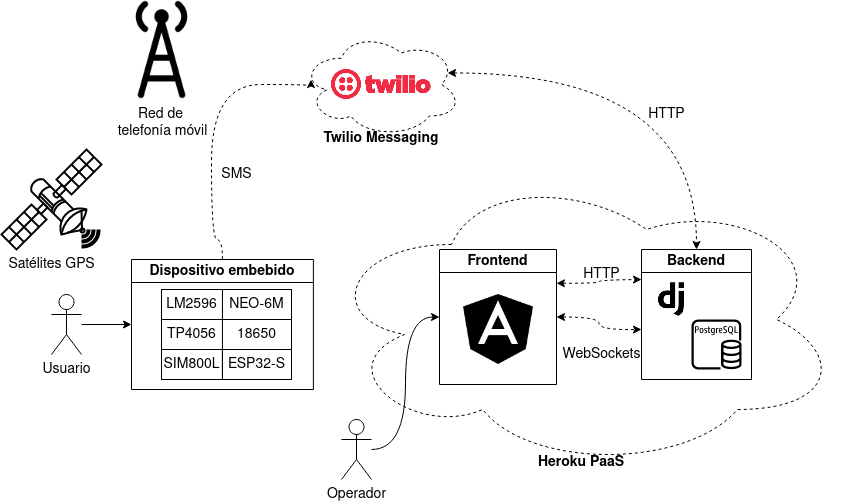
\includegraphics[width=1\textwidth]{./Figures/arquitectura.png}
	\caption{Arquitectura general del sistema}
	\label{fig:texmaker}
\end{figure}


Se pueden identificar los siguientes componentes:
\begin{itemize}
	\item En primer lugar, se observa a un usuario del dispositivo embebido, que es el componente que envía alertas mediante SMS hacia el servicio en la nube de Twilio.
	\item En segundo lugar, se encuentra el servicio de Twilio, que recepciona los mensajes recibidos y los reenvía mediante un \textit{webhook} hacia el servicio web o \textit{backend}. La comunicación entre el dispositivo embebido y Twilio fue posible ya que en este último se contrató un número teléfonico para la recepción de los SMS. 
	\item En tercer lugar, el \textit{backend}, que es el componente encargado de la recepción de alertas, procesamiento y almacenamiento de datos y comunicación con el \textit{frontend}. Fue desarrollado con el \textit{framework} Django, en Python.
	\item A continuación, se ubica el \textit{frontend}, que es la aplicación web que se encarga de toda la interacción del usuario operador con el sistema, incluyendo carga de datos y gestión de alertas. Consiste en una \textit{Single Page Application } y su desarrollo fue realizado en Angular, cuyo lenguaje es TypeScript.
	\item Por último lugar, se encuentra un componente menor, pero no menos importante que es la base de datos encargada de almacenar toda la información del sistema, como usuarios, alertas, tipos de alertas, entre otros. El motor elegido fue PostgreSQL, descrito en el capítulo anterior.
\end{itemize}
   
Resulta importante destacar que toda la interacción entre el \textit{backend} y \textit{frontend} es realizada mediante \textit{endpoints} HTTP y \textit{WebSockets} para comunicación en tiempo real, utilizando TLS/SSL para securizar las conexiones. 

Además, todos los \textit{endpoints} requieren de autenticación y autorización por parte del operador, a excepción de algunos que deben ser públicos para ser utilizados.

Por el lado del despliegue, los componentes web se desplegaron en la nube de Heroku mediante el uso de \textit{dynos} básicos, que son contenedores de aplicaciones web\citep{HEROKU:1}, y para la base de datos, se utilizó un \textit{addon} de PostgreSQL, que consiste en un complemento que permite incorporar una base de datos como SaaS u otros componentes requeridos por los sistemas, como pueden ser bases de datos en memoria o brókers\citep{HEROKU:2}.

\section{Desarrollo de módulos de hardware}

El firmware del dispositivo embebido fue desarrollado con el \textit{Espressif IoT Development Framework}, también conocido como \textit{ESP-IDF}, el framework oficial de la placa de desarrollo elegida para el proyecto, ESP32-S. Su lenguaje de programación es C y provee un robusto conjunto de bibliotecas para el desarrollo sobre periféricos y funcionalidades del ESP32. Adicionalmente, ESP-IDF funciona como registro de un conjunto de componentes realizados por el fabricante oficial o la comunidad para extender funcionalidades comunes de los sistemas embebidos. 

Como placa de desarrollo, el firwmare se desarrolló para una placa de desarrollo ESP32-WROOM-32s del fabricante NodeMCU, un kit de desarrollo atractivo por su bajo costo, interoperabilidad, documentación disponible y bajo consumo de energía. La ventaja de usar esta placa es que, además de contar con el framework ESP-IDF y todas las características descritas en el capítulo 2, permite que el firmware desarrollado pueda ser adaptado a placas de características similares, no quedando el firmware atado solamente a una alternativa.

Para el desarrollo, se importaron varias bibliotecas usadas para el desarrollo embebido. Entre estas, resulta importante destacar dos bibliotecas importantes:
\begin{itemize}
	\item \textit{libnmea}: Biblioteca que facilita la lectura de los datos recibidos del módulo GPS. Esto es posible ya que el NEO-6M utiliza un formato de mensajes estándar denominado NMEA. La ventaja de usar \textit{libnmea} es que convierte los datos recibidos en estructuras de C, pudiendo acceder rápidamente a valores como la latitud, longitud, etc.
	\item \textit{iot-button}: Biblioteca que permite configuraciones complejas sobre botones o pulsadores. La ventaja de utilizar este componente es que permite rápidamente configurar funciones de \textit{callback} ante eventos como pulsaciones largas, sin requerir que se desarrolle lógica de control, así como también contempla inconvenientes como un \textit{debounce} o falsas pulsaciones al momento de accionar el botón.
\end{itemize}

Estas dos bibliotecas fueron importadas al proyecto como \textit{managed components}, propios del registro de componentes externos de ESP-IDF. En la tabla \ref{tab:bibliotecas-esp32} se encuentra detallado el uso que tuvo cada biblioteca importadas para el firmware.

\begin{table}[H]
	\centering
	\caption[Tabla de bibliotecas]{Bibliotecas más relevantes utilizadas}
	\begin{tabular}{l c}    
		\toprule
		\textbf{Bibilioteca} & \textbf{Uso} \\
		\midrule
		\makecell{\textit{iot\_button.h}} & \makecell{Implementación del botón pulsador y acciones \\ a tomar al momento de ser usado } 	\\
		\hline
		\makecell{\textit{nmea.h}}	 & \makecell{Lectura de mensajes NMEA recibidos por el módulo GPS} 	\\		
		\hline
		\makecell{\textit{string.c}}  & \makecell{Manipulación y transformación de cadenas de texto \\ al momento de leer mensajes recibidos de los módulos}  \\
		\hline	
		\makecell{\textit{ctype.c}}  & \makecell{Uso de funciones comunes de C \\ para trabajar sobre caracteres de texto }  \\
		\hline
		\makecell{\textit{uart.h}}	 & \makecell{Comunicación con los módulos GSM y GPS \\ mediante puerto serie}	\\
		\hline	
		\makecell{\textit{esp\_system.h}} &  Funciones básicas del ESP-IDF\\
		\hline
		\makecell{\textit{esp\_log.h}} &  Visualización de errores y mensajes de \textit{debug} del firmware \\
		\hline
		\makecell{\textit{esp\_pm.h} \\ \textit{esp\_sleep.h}} & Configuraciones de ahorro de energía \\
		\hline
		\makecell{\textit{adc\_oneshot.h} \\ \textit{adc/adc\_cali.h} \\ \textit{adc\_cali\_scheme.h}}  & \makecell{Conversión del módulo analógico-digital y lectura \\ de valores para calcular la carga de la batería} \\
		\hline
		\makecell{\textit{nvs.h} \\ \textit{nvs\_flash.h}} &  \makecell{Almacenamiento \textit{flash} para guardar datos  en la \\ memoria no volátil, como la última posición válida} \\
		\hline
		\makecell{\textit{freertos/FreeRTOS.h}} & Configuración del sistema operativo en tiempo real \\
		\hline
		\makecell{\textit{freertos/task.h}} & Implementación de procesos/tareas \\
		
		\bottomrule
		\hline
	\end{tabular}
	\label{tab:bibliotecas-esp32}
\end{table}

Para el desarrollo, compilación, pruebas y monitoreo, se trabajó con el entorno de desarrollo integrado Visual Studio Code, en conjunto con la extensión oficial de ESP-IDF, el cual facilita el trabajo con el kit de desarrollo y la incorporación y uso de módulos propios del ecosistema del ESP32. En la figura \ref{esp32:diagrama} se pueden observar los componentes físicos del dispositivo embebido:


\begin{figure}[H]
	\centering
	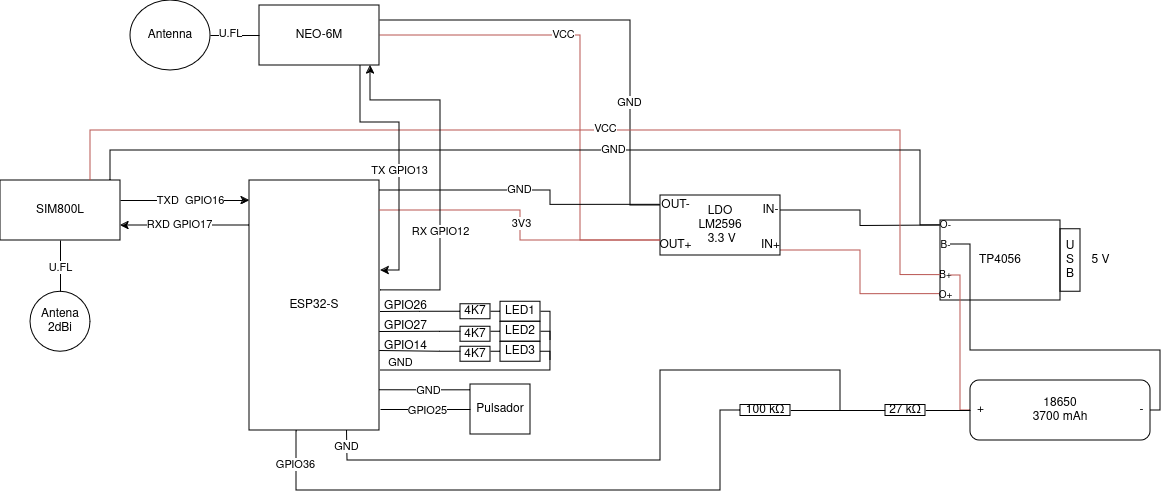
\includegraphics[width=1\textwidth]{./Figures/esp32-arquitectura.png}
	\caption{Esquema de componentes de hardware del ESP32}
	\label{fig:esp32:arquitectura}
\end{figure}

Adicionalmente a los dispositivos originalmente elegidos, se incorporó un regulador de tensión LM2596 en la entrada de energía de la batería no contemplado originalmente, con el objetivo de adecuar el voltaje de entrada de 4.2 V a 3.3 V. Además, se incorporó una antena activa para el módulo GPS ya con una antena pasiva la precisión de la localización obtenida era baja o tomaba más tiempo del esperado. Por otra parte, se reemplazó la antena helicoidal del módulo GSM por una con formato PCB y 3dBi de ganancia.

\subsection{Tareas del dispositivo embebido}

Para implementar las funciones del dispositivo embebido, se dividió el desarrollo del firmware en 7 bloques o funciones de código principales. Estas se pueden describir de la siguiente forma:

\begin{itemize}
	\item Inicio: consiste en la función de arranque del firmware, en donde se realizan acciones como inicialización de periféricos, revisión de errores de arranque, reducción de la velocidad de reloj del procesador al mínimo requerido, asignación inicial de variables, y por último, la configuración de las tareas que corren en bucle. Posterior al inicio, esta función finaliza su ejecución. En la figura \ref{fig:esp32:tasks1} se pueden observar todos los pasos contemplados. No es una tarea en el sentido estricto de \textit{FreeRTOS}.
	\item Manejador del módulo GSM: consiste en una función con un bucle infinito que se encarga de cada pocos segundos recibir comandos/respuestas del módulo SMS leyendo el puerto serie y tomar una acción ante cada mensaje si corresponde. En la figura \ref{fig:esp32:tasks1} se puede visualizar el bucle con las acciones que realiza. Los mensajes manejados son:
		\begin{itemize}
			\item \texttt{AT}: mensaje que representa un OK.
			\item \texttt{CMT}: mensaje que significa que se recibió un SMS; esto se utiliza para configurar el número de teléfono al cual se le deben enviar las alertas por SMS.
			\item \texttt{CMGS}: mensaje que significa se envió correctamente un SMS; se utiliza para confirmar el envío correcto de una alerta.
			\item \texttt{CSQ}: mensaje que incluye el nivel de calidad de la señal de telefonía móvil.
			\item \texttt{GSN}: mensaje que incluye el IMEI del dispositivo; se utiliza como mecanismo de seguridad ya que el SMS de configuración de teléfono debe incorporar los primeros dígitos del IMEI como validación.		
		\end{itemize}
		\item Manejador del módulo GPS: consiste en una función con un bucle que se encarga de recibir comandos/respuestas del módulo GSM leyendo el puerto serie y guardar la información recibida. Existen diferentes tipos de mensajes, pero para los fines del registro de la localización, solamente se está guardado la información del tipo de mensaje \textit{GPGGA}, que informa la posición actual y datos de los satélites\citep{nmea:1}. En la figura \ref{fig:esp32:tasks1} se puede visualizar el bucle con las operaciones.
		\begin{figure}[H]
	\centering
	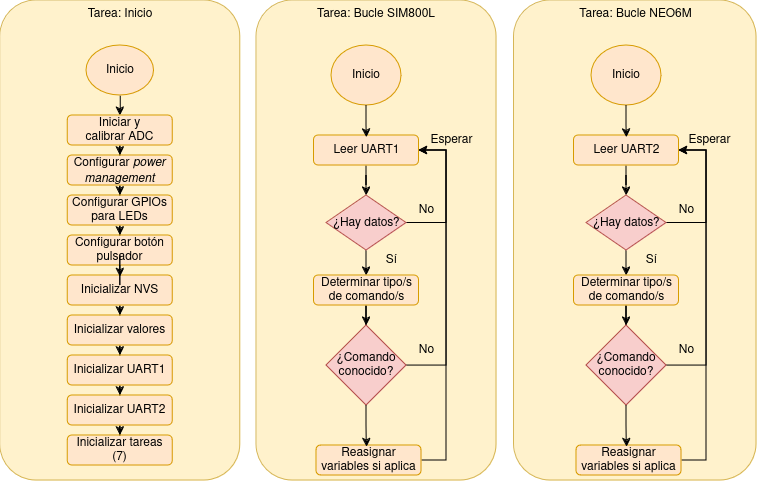
\includegraphics[width=0.95\textwidth]{./Figures/esp32-tasks1.png}
	\caption{Diagramas de flujo de tarea inicial, y bucles del módulo GSM y GPS}
	\label{fig:esp32:tasks1}
\end{figure}
		\item \textit{Setup} de energía del módulo GSM: tarea que espera por la correcta inicialización del módulo GSM y posteriormente, aplica algunas optimizaciones de energía. En la figura \ref{fig:esp32:tasks2} se listan los pasos ejecutados. Luego, la tarea termina su ejecución.
		\item \textit{Setup} de energía del módulo GPS: tarea que espera por la inicialización del módulo GPS y comunicación con al menos 5 satélites para enviarle algunos comandos de optimización. Luego de esto, la tarea finaliza. En la figura \ref{fig:esp32:tasks2} se pueden visualizar el flujo de esta.
		\begin{figure}[H]
	\centering
	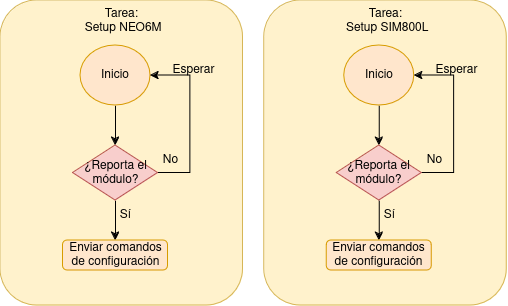
\includegraphics[width=0.75\textwidth]{./Figures/esp32-tasks2.png}
	\caption{Diagramas de flujo de las tareas de \textit{setup} de energía}
	\label{fig:esp32:tasks2}
\end{figure}

		\item Control de estado de GPS, GSM y batería: esta tarea tiene como objetivo, cada 30 segundos, leer el estado de las variables de calidad de la señal GSM, cantidad de satélites conectados y nivel de batería, y parpadear 3 luces dependiendo del estado de estas variables. En el desarrollo, se repartió en tres funciones pequeñas, pero a fines explicativos se presenta como una única tarea. En la figura \ref{fig:esp32:tasks3} se puede observar el flujo de ejecución de la tarea.
		\item Almacenamiento períodico de datos: cada 1 minuto esta tarea se encarga de leer las variables de latitud, longitud, IMEI y número de teléfono asignado y almacenarlas en el almacenamiento no volátil. en el caso de que los valores fueran válidos. En la figura \ref{fig:esp32:tasks3} se puede observar el bucle ejecutado por la tarea.
		\item Control períodico del módulo GSM: esta tarea se encarga de solicitarle información al módulo GSM información sobre el estado de la red cada 1 minuto. Esto es debido a que el módulo GSM no reporta automáticamente su estado, a diferencia del módulo GPS que si lo hace.  En la figura \ref{fig:esp32:tasks3} se puede apreciar el control que realiza la función.
		
				\begin{figure}[H]
	\centering
	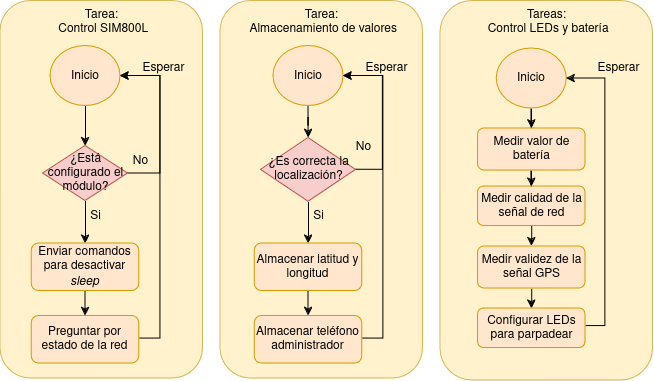
\includegraphics[width=0.9\textwidth]{./Figures/esp32-tasks3.png}
	\caption{Diagramas de flujo de las tareas de control y almacenamiento}
	\label{fig:esp32:tasks3}
\end{figure}

\end{itemize}


Por último, se puede considerar una última función más dentro del firmware que es el interruptor ante la pulsación del botón activador. En caso que se supere un umbral de 3 segundos del pulsador presionado, se activará \textit{callback} definido para ese evento. Este evento se encarga de levantar los valores actuales de la última localización válida almacenada, determinar cual es el número de teléfono al cual se debe enviar el mensaje de alerta y enviar los comandos hacia el módulo GSM para enviar el SMS. 

En la figura \ref{esp32:callback} se muestra un diagrama de flujo resumido de la operatoria de la interrupción. Para la asociación del \textit{callback} con el evento, se puede ver el código definido en la función inicial del firmware en la figura \ref{esp32:callback-codigo}, donde \texttt{sos\_button\_long\_press\_cb} es una función definida y \texttt{cfg} es la definición del evento.

\begin{lstlisting}[label=esp32:callback-codigo,caption=Definición del evento y asociación del \textit{callback}]  % Start your code-block
// SOS button configure
button_config_t gpio_btn_cfg = {
    .type = BUTTON_TYPE_GPIO,
    .long_press_time = SOS_BUTTON_LONG_PRESS_TIME_MS,
    .gpio_button_config = {
        .gpio_num = SOS_BUTTON,
        .active_level = 1,
        .enable_power_save = true},
};

button_handle_t gpio_btn = iot_button_create(&gpio_btn_cfg);
if (NULL == gpio_btn)
{
    ESP_LOGE(TAG, "Button create failed");
}

button_event_config_t cfg = {
    .event = BUTTON_LONG_PRESS_START,
    .event_data.long_press.press_time = SOS_BUTTON_LONG_PRESS_TIME_MS,
};

ESP_ERROR_CHECK(iot_button_register_event_cb(gpio_btn, cfg, sos_button_long_press_cb, NULL));

\end{lstlisting}

\begin{figure}[H]
	\centering
	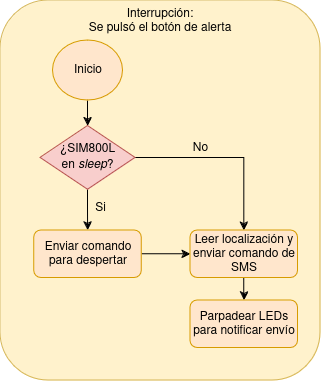
\includegraphics[width=0.75\textwidth]{./Figures/esp32-callback.png}
	\caption{Diagrama de flujo del \textit{callback} por pulsación}
	\label{fig:esp32:arquitectura}
\end{figure}


\subsection{Optimizaciones de energía aplicadas}

Se aplicaron diferentes técnicas de optimización sobre el ESP32-S y los módulos GSM y GPS con el objetivo de optimizar y disminuir el consumo de energía:
\begin{itemize}
	\item Se configuró \textit{FreeRTOS} para solamente utilizar un núcleo del ESP32-S.
	\item Se limitó la frecuencia del procesador para solamente utilizar como máximo 80 MHz.
	\item Se desactivaron todos los periféricos no usados, como WiFi, Bluetooth, etc.
	\item Se configuró el \textit{Dynamic frequency scaling} o DFS del ESP32, que permite que el 
	\item Se configuró el modo \textit{sleep} del módulo SIM800L, desactivandolo solamente cada ciertos intervalos de tiempo.
	\item Se desactivó el LED de notificación de calidad de señal del módulo SIM800L, ya que la comprobación se realiza de forma programática.
	\item Se redujo la frecuencia de actualización de mensajes del módulo NEO-6M hacia el ESP32.
	\item Se aplicó sobre NEO-6M una configuración de energía llamada \textit{Power Save Mode} para reducir la frecuencia de actualización hacia los satélites GPS.
	\item Se configuró el modo \textit{sleep} del módulo SIM800L, desactivandolo solamente cada ciertos intervalos de tiempo.
	\item Se utilizaron tiempos muertos de espera o \textit{standy} del orden de varios segundos en el ESP32-S para permitir reducir la frecuencia, resultando en que gran parte del tiempo la placa se encuentra en espera.
	\item Se redujo el consumo de energía de los 3 LEDs indicadores de GSM, GPS y batería mediante la incorporación de resistencias, requiriendo aproximadamente 1 mA para todos los LEDs.
\end{itemize}

Adicionalmente, se intentó aplicar un manejo tanto manual como automático (configurable mediante el uso de DFS) del modo \textit{light sleep} pero se encontró que, después de varios intentos y pruebas, el consumo de energía no disminuyó. Esto es debido a características de fabricación del modelo ESP32-WROOM-32s de NodeMCU, como el regulador de tensión incorporado en la placa de desarrollo, que tiene un consumo en \textit{idle} de aproximadamente 15 mA, aunque esté en \textit{deep sleep} o \textit{light sleep}.

Además, la incorporación de \textit{light sleep} complejiza la lógica de funcionamiento de las tareas del ESP32, y siendo que no se pudo verificar la reducción de consumo energético al utilizarlo, se descartó. Por último, se notaron algunos inconvenientes al momento de leer datos de los módulos UART. En caso de haber continuado con la implementación del modo \textit{light sleep} de forma automática, hubiera sido necesario incorporar algunas comprobaciones adicionales para solucionar esta inestabilidad. La ventaja de utilizar el modo automático de \textit{light sleep} es que gran parte del tiempo \textit{idle} del ESP32 hubiera representado un ahorro de energía de varios mA.

\section{Desarrollo de módulo de backend}

El \textit{backend} fue desarrollado con el framework Django y Python. Para todas las funcionalidades, se estructuró el proyecto siguiendo los lineamientos de Django, que consiste en principalmente dividir la aplicación en módulos web por temática o características. Para el caso de esta aplicación, se identificaron dos módulos:
\begin{itemize}
	\item \textit{Users}: para englobar toda la funcionalidad referida a usuarios.
	\item \textit{Alerts}: para englobar toda la funcionalidad referida a usuarios.
\end{itemize}

Esto no significa que no puedan o no deban referenciarse los módulos entre sí, sino que es una forma lógica de estructurar la información perteneciente a la misma lógica de negocio. En la figura \ref{backend:folder1} y \ref{backend:folder2} se pueden visualizar las carpetas de cada módulo con sus respectivos componentes.

\begin{figure}[H]
\centering
\begin{minipage}{.5\textwidth}
  \centering
  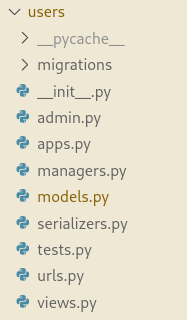
\includegraphics[width=.4\linewidth]{./Figures/backend-folder1.png}
  \captionof{figure}{Estructura de archivos de módulo de \textit{Users}}
  \label{backend:folder1}
\end{minipage}%
\begin{minipage}{.5\textwidth}
  \centering
  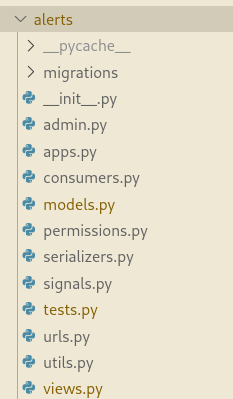
\includegraphics[width=.4\linewidth]{./Figures/backend-folder2.png}
  \captionof{figure}{Estructura de archivos de módulo de \textit{Alerts}
  \label{backend:folder2}
\end{minipage}
\end{figure}


Respecto a las características, se diseño el \textit{backend} con la idea de un producto \textit{multitenant}, es decir que permita que a futuro existan diferentes organizaciones cliente dentro de este. Debido a esta característica, todos los datos están contenidos dentro de una misma organización, compartida por los usuarios, beneficiarios, entre otros datos cargados. En la figura \ref{backend:modelo} se puede visualizar el modelo de datos relacional con las entidades diseñadas.

\begin{figure}[H]
	\centering
	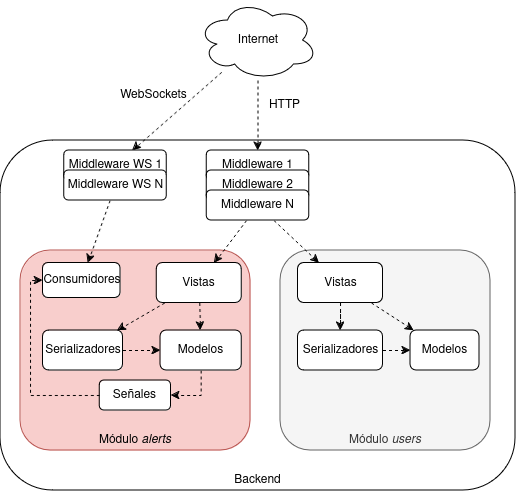
\includegraphics[width=0.75\textwidth]{./Figures/backend-modelos.png}
	\caption{Modelo de datos}
	\label{backend:modelo}
\end{figure}

De todas maneras, para esta versión inicial, solo se contempla un usuario por organización en el \textit{frontend}, aunque a futuro el diseño y la lógica de negocio en la API se encuentra desarrollada para contemplar una organización con un usuario raíz o padre y un conjunto de usuarios operadores, de menor privilegio.

\subsection{Seguridad}


Servicios desarrollados

\section{Desarrollo de módulo de frontend}

\section{Integración}}
